%%% Thesis Introduction --------------------------------------------------
\chapter{INTRODUCTION}
\label{chap:intro}

\graphicspath{{Introduction/IntroductionFigs/EPS/}{Introduction/IntroductionFigs/}}
\nomenclature[z1]{\cms}{Character Motion Synthesis}
\nomenclature[z2]{\cpg}{Central Pattern Generator}
\nomenclature[z3]{\dof}{Degree of Freedom}
\nomenclature[z2]{\moit}{Motor Invariant Theory}

\section{The Challenge}
Character Motion Synthesis (\cms) research aims at generating motion for virtual characters.
It is a topic of significant value in theory and application. 
Besides major applications in the media industry, where both computer games and animation films depend heavily upon character motions for storytelling, 
current applications also include  areas like user interface design, psychology, sports and medicine.

The challenge of \cms  is not to make characters move, but  to make them lifelike. 
Underneath this challenge is human's marvellous ability of motion perception. 
In real life, motions are very similar; 
while from the varieties in motion details, humans can infer mental states, health conditions or the surrounding environment.
%\note{uncanny valley}
A famous psychological phenomenon is the ``uncanny valley''.
For characters with realistic human-like appearance, slightly artefacts in motions may result a strong emotional revulsion.



Nowadays in industry, high quality motions are mainly generated by manual work. 
Very often, characters are complex and contain a large number of joints, making animation a tedious work.
Making it worse, reusing motion animation is also difficult and prone to artefacts.
High level animation tools are badly needed. 

%\note{Do An introduction for physicall based animaiton?}
Real life motions highly interact with the environment.
Physics based method  is most important research endeavour at current.
Besides  the addition of the dynamic interactive responses, it is  expected  the elimination of  artefacts that violating physics  will make motions more natural looking.
However, this paradigm faces many difficulties, mainly computational cost and modelling difficulty.
In fact, such problems has been identified by biological researchers earlier.


Motion closely relates to perception.
Environment perception is foundation of motor control.
Phenomena such as  ``uncanny valley '' pose  important questions for perception. 
Some awkward artefacts are spotted instantly even they are physically feasible, while many physical impossible motions are accepted as realistic and entertaining. 



Difficulties in \cms reflects the inferiority of artificial control method.
The peculiarity of motion perception and control suggests  biological systems may adopt a different principle.
This thesis is founded on new paradigms in biological research.

 

\section{Agile Animals}
%\note{Underlying these problems} is our misunderstanding of animal motions.
Although animals have fascinated us for thousands of years, we still don't fully understand how they move.
Animals are very different from artificial machines and such comparisons may reflects the  biological motor control principle.
%some basic questions of motor control and motion perception remain open. 
%And answers to such questions become even more valuable nowadays. 
%Advance in this topic will greatly influence the biology, robotic engineering even intelligent research.
%\note{The difference between biological motor system}

%The paradoxes is even human are good at motor control and motion perception; human still don’t have an idea of how we move and how we perceive motion.
%Before going into details into the research ideas, we first review some puzzles troubles the foundation of CMS. 
\begin{itemize}
\HiItem {Degrees of freedom ({\dof}s)}.
From Mechanical perspective, animals have many more {\dof}s than their artificial counterparts.
An artificial ship can be approximated by a simple rigid body; while a fish has the flexible vertebrae of tens of {\dof}s.


In principle, the extra {\dof}s admit more variations for adapting the environment. 
But for the control system, too many extra {\dof}s is a disaster for the computational burden. 
For a human to take one step,  the neural system controls more than $600$ muscles .
With nowadays computer, solving the dynamics directly will require inhibitive computational time.

 
\HiItem {Versatility}
Most artificial machines are designed with a single purpose,while animals are capable  of unlimited tasks.
Many biological functions which often neglected by \cms research, such as the feeding, breeding, language and vision, depend on motor control. 
Besides walking, swimming and many other styles of locomotion , we utilize many tools, such as cars, skate, bicycle and tennis.

Follow tradition control ideas, it seems unlimited resources are allocated for unlimited number motion controllers, while biological research shows motor control cost very little mental resources.

\HiItem{Performance}
Although the problem of biological motor control is more complex , the resulting performance surpasses artificial machines in many aspects.
Natural motion are more
\begin{enumerate} 

\HiItem{Robust:}
Human can maintain walking stability on tough terrains inaccessible for vehicles.

\HiItem{Manoeuvrable and speedy:}
Typical modern aeroplanes will travel $32\: body\: lengths/sec$ and yaw $720\: deg/sec$ at max.
while pigeons may travel $75 \:body\: length / sec$, yaw at about more than $5000 \: deg/sec$.

\HiItem{Energy Efficient:}
The energy consumed by human walking is only $5\%$ of that for the world famous humanoid ASIMO.
\end{enumerate}

\end{itemize}



%For computer animation research, the key principle is we should know the things we animate.
%Natural motion system has many valuable properties which are not captured by current motion synthesis methods.
%\begin{itemize} 
% \HiItem{robust}
%Natural motions are adaptive to the changes in the environment or body conditions. 
%A common example is human locomotion. 
%Walking on different terrains will exhibit different gait while the balance is maintained. 
%
%\HiItem{speedy}
%Some motions of animals are very fast, honey birds may vibrate their wings in kHz.
%The astonishment is to the speed of motion, more puzzling is that the neural system can solve the complex motion control problem in such a short time. 
%When an animal avoids obstacles at very high running speed, 
%it must continue its running, make a turning and keep balance at the same time. 
%It seems easy for the neural system to plan complicate motions.
%\HiItem{Energy Efficient}
%Natural Motions are energy efficient.
%In theory, this idea is supported by Darwin's Theory of Evolution.
%But animals spent far less energy than our expectation.
%An example is that the energy consumed by human walking is only 5\% of that for a robot of the same scale.
%\end{itemize}

\section{Motor Invariant Theory}
Biological Motor Control achieved a delicate balance of robustness, controllability and energy efficiency.
The real-time performance may further suggest that the biological method  is simple and requires little computational load.
These are the dreaming properties for \cms research and  explanation from biological research forms the gene of the thesis.


\subsection{Different Biological Idea}
\begin{itemize}
\HiItem {Role of Control and Computational Burden}
Many procedural \cms methods separate ``motion'' and ``force''  planning.
A motion trajectory is planned first and then force are planned to drive the character to follow the motion curve.
Two many redundant {\dof}s that spoil this approach  with inhibitive computational cost.

As an alternative, some researchers have proposed the memory based model for motor control and developed data-driven methods.
But such methods lacks the versatility and adaptivity.
Unlimited memory is needed for motion data  and searching in the ever increasing database becomes more and more challenging.



In real life, when force is determined, motion trajectory is determined.
Many biological researchers have suggested that there is no motion-force separation in planning,
some researchers even  propose that the forces are not directly calculated.
A suggestion is  the neural system plays only a limit function in motor control.
It is the body and environment that play the crucial role, their dynamic interactions form some  patterns or templates for motion.
The neural system only tweaks the basic templates for specific purpose.



 
 
	
\HiItem{Feedback or Feed-forward}
Most artificial control methods follow the principle of feedback.
Control are applied to track the target and counteract perturbations.
This method is also called ``shooting'' or ``tracking''.


Many  biological researchers believe that motor control is feed-forward based and relies on experience.
If perturbations can be predicted, measures are taken beforehand to prevent ``failure''.
The prediction nature also suggest motion trajectory can not be controlled in precision.
 


\HiItem{Natural Dynamics} 
In the feedback framework, natural dynamics effects are treated as perturbations and are cancellated by the control input.

From the biological perspective, the mechanical structures are product natural selection which evolve with the environment for millions of years. 
They are advantages rather than handicap. 
Some researchers believe biological motor control limit the control input and explore the natural dynamics.
\end{itemize}


\subsection{Motor Invariant Theory}
%In this thesis, we propose different idea towards motor control and motion synthesis.
%In this research, we propose a different motion synthesis method based on a different motor control theory.
%
%An insightful discovery is that motor control can be “easy”.
%For some situation, some tasks mainly explore the properties of the body and environment and can be achieved with little control effort.
%In nature, we don’t finish difficult motion tasks, we select many easy motion tasks that we are good at, connect or modify them for our special purpose.
%
%The “easy” tasks are called motion primitives; they are the basic elements of our motor ability. 
%When we modify the motion primitives, some valuable properties of motion primitives are kept unchanged, and the maintained properties are called motor invariants.
%
%The inspiration of our idea comes from related biological research, which covers biomechanics and neural science.





This thesis proposes a new idea for the adaptivity and versatility of motion.
For motions in different scenario, some dynamics properties are invariant and some properties are variable.
The conjecture is that: rather than detect and cancellate all kinds of perturbation, biological motor control relies on the property invariance for motion success.
This idea is named as \emph{Motor Invariant Theory(\moit)}.
From dynamic perspective, such properties are stable.

\moit incorporates the motion primitive conjecture. 
Motion Primitives are the template dynamic systems that are stable.
The remaining question is how to utilize the templates synthesized new motions.

The \moit propose that when facing a new situation, human don't solve motor control from ground up,
we try to utilize  successful experience in similar situation.
Controlled motion dynamics are qualitative the same with the motion primitives or templates.
The topology conjugacy are introduced to model the similarity in dynamics.

In dynamic motion synthesize research, a motion is represented by $x(t)$, which is a solution to the body and environment dynamics(Equation ~\ref{eq:BodyEnvDym}).
\begin{equation}
\dot{x}=F(x)
\label{eq:BodyEnvDym}
\end{equation}


Suppose Equation~\ref{eq:BodyEnvDym} is used to describe a motion primitive or template dynamic system,
 we can define a transformation $T$ that acts on the space of $x$.
\[
\tilde{x}=T(x)
\]
then we can obtain two equations in  the transformed state $\tilde{x}$ (Equation ~\ref{eq:tranformedEQ} )and original state $x$(Equation ~\ref{eq:EQtransform}).

\begin{equation}
\dot{\tilde{x}}=F(\tilde{x})
\label{eq:tranformedEQ}
\end{equation}

\begin{equation}
\dot{x}=\tilde{F}(x)
\label{eq:EQtransform}
\end{equation}

These two equations describe the same motion but in different coordinates.
From one solution, we can get another solution by transformation.
Suppose $x'(t)$ is the solution to Equation~\ref{eq:EQtransform} and $\tilde{x}(t)$ is the solution to the Equation~\ref{eq:tranformedEQ}
\[
x'(t)=T^{-1}(\tilde{x}(t))
\]
Equation~\ref{eq:tranformedEQ} and Equation~\ref{eq:BodyEnvDym} are the same, thus we have
\[
\tilde{x}(t)=x(t)
\]
Then we have
\[
x'(t)=T^{-1}(x(t))
\]




%if we substitue x=f(x,t) into (1).
%we can express equation (2) interm of (x,t,x)
%\dot(x)=F'(x).
%then the solution of the equation becomes 
%x2(t)=(x)t=f-1(xt)
%
%
The  transformation method has many advantages.
It has much less computational burden and maintains many important properties.
If the original system is stable, then the transformed system is also stable.
%
%
From geometrical perspective, a dynamic equation assign a vector $\dot{x}$ to each position $x$, which is called vector field.
If there exist continuous one-one mapping between the two vector field, then the two vector field  or dynamic equation are \emph{topological conjugate}.
This relationship is presented by $F \simeq \tilde{F}$.
$F$ and $\tilde{F}$ are called \emph{analogous systems}.
The conclusion is necessary and sufficient.
If two systems are the topologically conjugate ,then there is an one one mapping between the states.
Thus there are two method for motion adaptation.

If the perturbation does not violate the topology, the corresponding one-one mapping will modify the motion.
From dynamic perspective,the topology preserving ability is an intrinsic property of many dynamic systems:
\emph{structural stability}.
For motor control, methods are taken to maintain the topology or enhance the structural stability.
In many situation, we only know the qualitative property are preserved and the existence of the one-one mapping.
But find out details of motion will be difficult or computational expensive.
This strategy is qualitative.
In \moit, this theory explain the involuntary motion adaptation and the effects of low level neural control system.

The topological structure is one important motor invariant: the \emph{Global Motor Invariant}.
Global Motor Invariant determines the stability of motions.
Not only by perturbation, motion adaptation can also be generated by adjusting system parameters, which are \emph{System Adaptations}





Also if the transformation is known, then the two systems must be topological equivalent.
In many situation, to achieve desired transform $T$, control effort needed to be applied.
This method  modifies motion with precision and \moit apply this idea for high level voluntary motor control.
For this method, chose a proper transformation $T$ is the most challenging  question.

In \moit, selection of $T$ is based on two principles.
\begin{itemize}
\item
Parameters of transformation $T$ should be easy to detect and formulated, which meets the biological sensing and computational constraints. 

\item 
The transformation $T$ should be energy efficient.
For differential dynamic system, some transformation explore the natural dynamics and requires little or no energy input.
\end{itemize}

Some quantitative properties will be unchanged during transformation, which are called \emph{Local Motor Invariant}
Motion Adaptations that are precise and voluntary controlled are called \emph{Transform Adaptation}





%the stability of the orignal system is known.
%if possible, we always try to tranform the stable motion.
%To this end motor control are applied to execute the transformation
%
%
%
%these two ideas have pros and cons.
%The first method maintail the qualitative properties, but details of motion can not be controlled precisely.
%if the second method is applied, given the transformation, the resulting motion can be know, while but to carried out such transformation, controll effort may needed.
%
%




Although new mathematical tools seem obscure at first glimpse.
The underlying idea is intuitive and can be explained well by commonly observed phenomena.



\subsection{The Floating Ship: An example of Stability}
The floating ship  example shows the idea of structural stability and topological conjugacy.
In real life, ships floating on the wave, are typically taller than they are wide,as shown in Figure~\ref{fig:ShipFloating}.
The  question is how the ship maintain its posture.

Through analysing the topology and structural stability, we see that it is trivial to maintain posture.
This conclusion applies to different ships for their dynamics are qualitative the same, or topological conjugate.


\subsubsection*{Dynamics}

\begin{figure}[!htbp]
  \begin{center}
    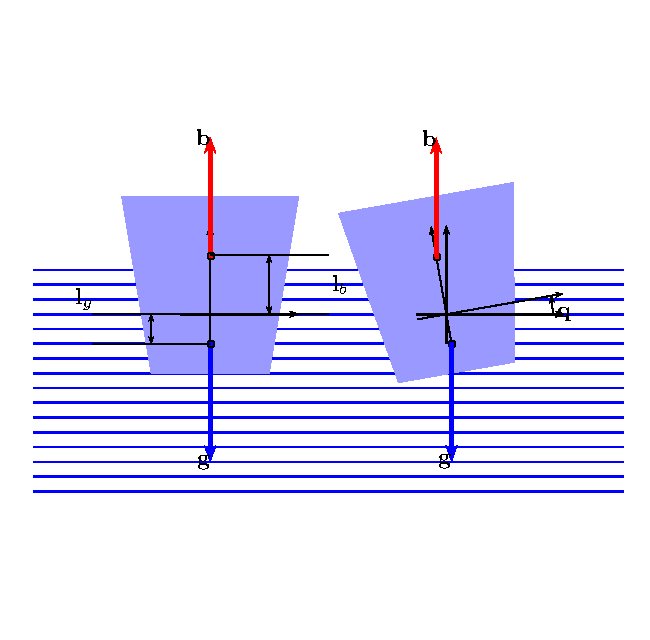
\includegraphics{ShipExample}
    \caption{The Floating Ship Example}
    \label{fig:ShipFloating}
  \end{center}
\end{figure}

The sway motion shown in Figure ~\ref{fig:ShipFloating} is described by Equation~\ref{eq:shipflow}
\begin{equation}
\label{eq:shipflow}
J\ddot{q}+d\dot{q}=\tau(q)_{g}+\tau(q)_{b}+\tau_{u}
\end{equation}

When the ship floating on the sea, motion is governed by the two forces, the buoyancy $b$ and gravity $g$.
$q$ is the swaying angle.
$J$ is the inertia,  
$d$ is the damping coefficient,
$\tau_{g}$,$\tau_{b}$,$\tau_{u}$ are the corresponding the torques of gravity, buoyancy and external control.
When $\tau_{u}=0$,  the floating ship  becomes an \emph{autonomous system} governed by natural dynamics.

To make it consistent with discussions in following chapters, Equation~\ref{eq:shipflow} is reformulated.
Define the \emph{state} variable $\state=[q,\qd]$, Equation~\ref{eq:shipflow} becomes
\[
\dot{\state}=F_{J,d}(\state)+Du
\]

where 
$F$ is a function of $\state$, the subscripts~$J$ and~$d$ are \emph{system parameters}.
$D$ is a matrix,which describe how the control effort is applied.
$u$ is \emph{control input}, for this example is $\tau_{u}$



\subsubsection*{Equilibrium Postures}
A ship will only rest when $\tau_{g}+\tau_{b}+\tau_{u}=0$, which are called \emph{Equlibrium} Postures.
The only two possible ones are show in Figure ~\ref{fig:ShipEqulibriumStable} and Figure~\ref{fig:ShipEqulibriumUnstable}
\begin{figure}[!htbp]
  \begin{center}
     \includegraphics{leftPos}
    \caption{The Stable Equilibrium Posture}
    \label{fig:ShipEqulibriumStable}
  \end{center}
\end{figure}

\begin{figure}[!htbp]
  \begin{center}
     \includegraphics{rightPos}
    \caption{The Unstable Equilibrium Posture}
    \label{fig:ShipEqulibriumUnstable}
  \end{center}
\end{figure}



The two postures are different, illustrated with the \emph{phase plot}.
On the phase plot, the horizontal axis represents  $q$; and the vertical axis represents velocity $\qd$. 
The motion of the ship is shown as a curve on the phase plot, which is called \emph{flow}.

The posture in Figure ~\ref{fig:ShipEqulibriumStable} is \emph{attractive} or \emph{stable}.
If a small perturbation moves the ship away from the left posture, it will return to the equilibrium posture automatically as shown in Figure~\ref{fig:StablePosture}.
\begin{figure}[!htbp]
  \begin{center}
      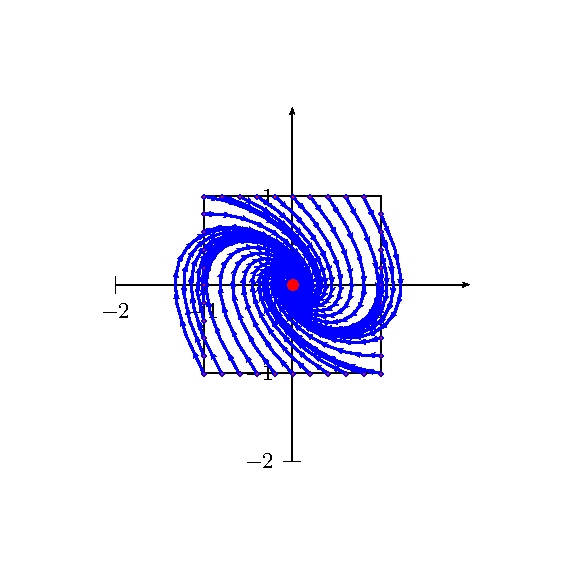
\includegraphics{stablePosition}
    \caption{Phase Plot of the Stable Posture}
    \label{fig:StablePosture}
  \end{center}
\end{figure}


The  posture in Figure~\ref{fig:ShipEqulibriumUnstable} is \emph{repelling} or \emph{unstable}.
Away from the equilibrium posture, it will move away further, as shown in Figure~\ref{fig:unStablePosture}.

\begin{figure}[!htbp]
  \begin{center}
      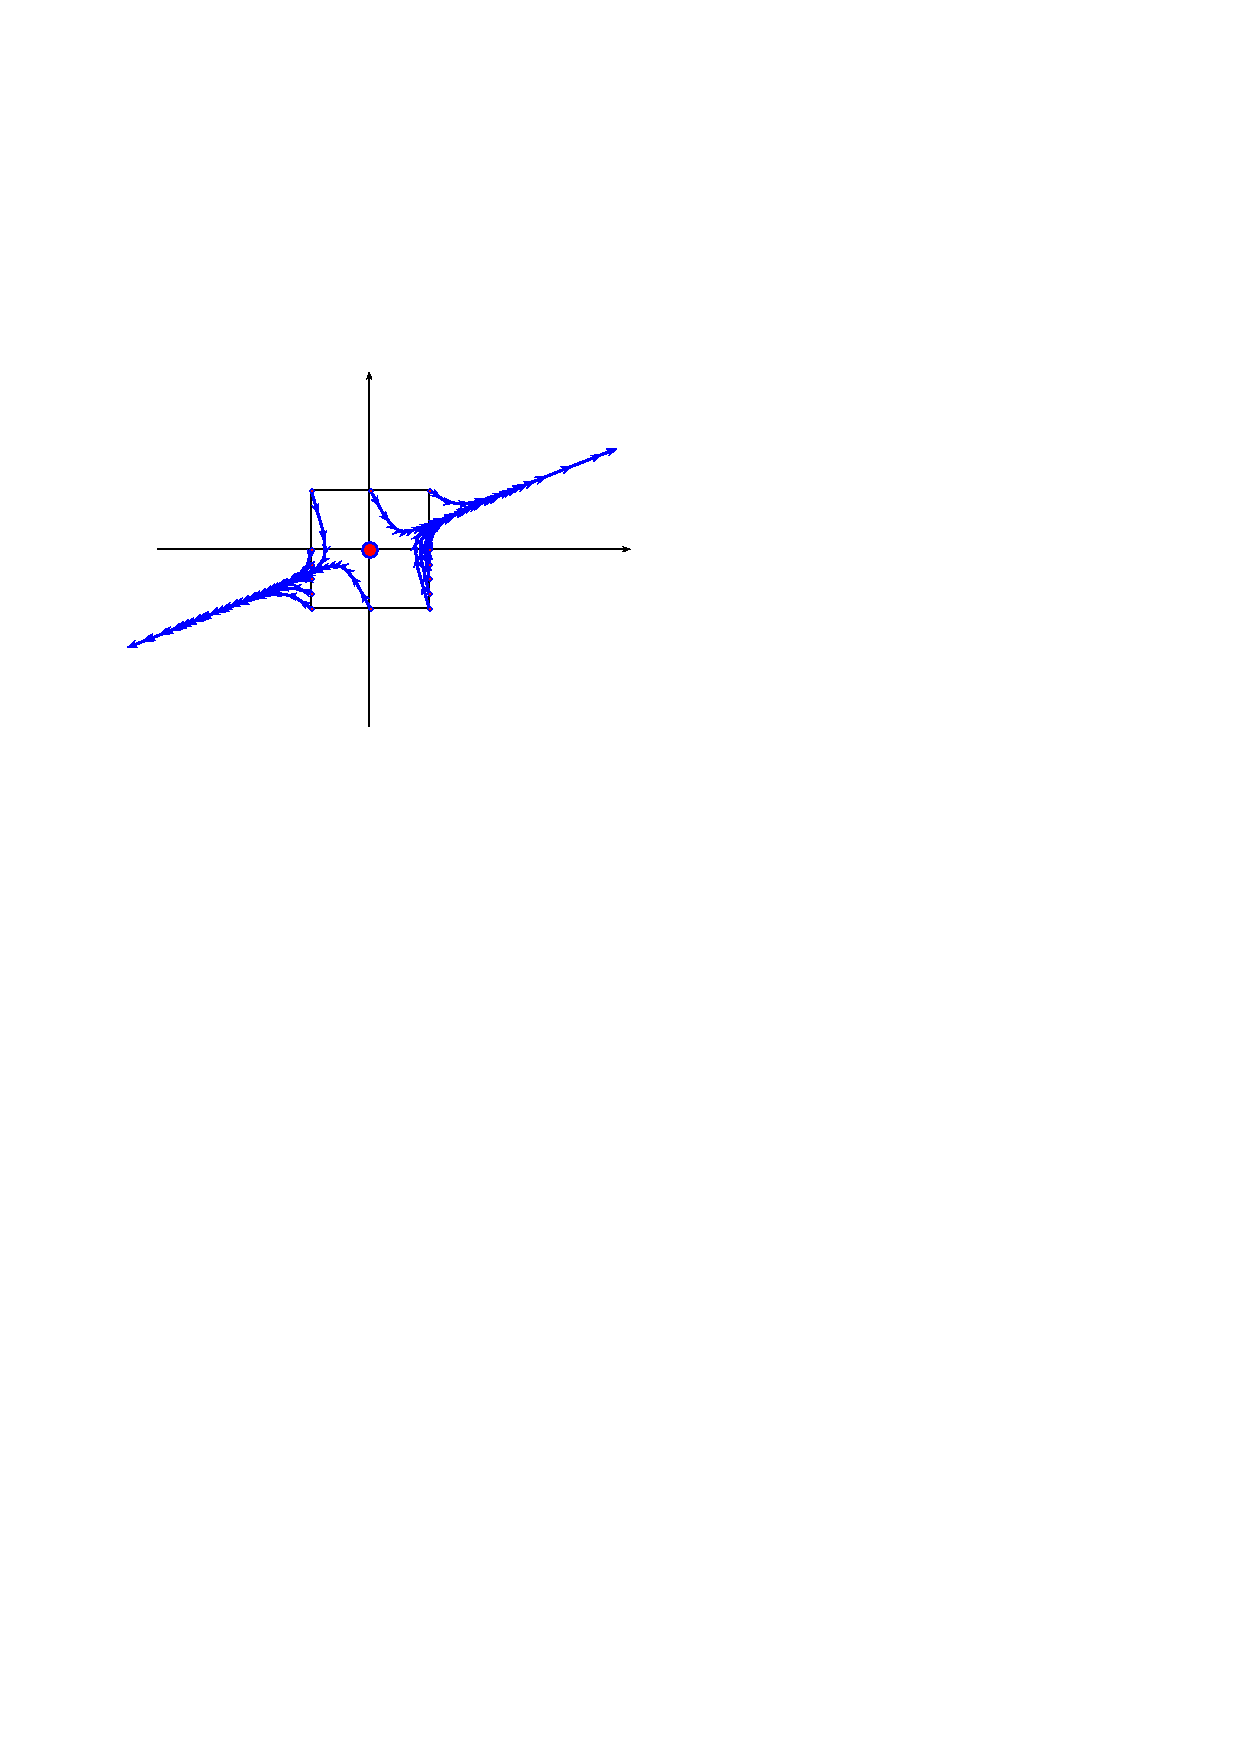
\includegraphics{unstablePosition}
    \caption{Phase Plot of the Unstable Posture}
    \label{fig:unStablePosture}
  \end{center}
\end{figure}


\subsubsection*{Trivial Task}
All the flows form the \emph{phase portrait} of the dynamic system. 
The discovery is that all the flows start from the repelling posture and ends at the attractive posture.
Several example curves are show in Figure ~\ref{fig:globalflow}

The attractive posture is maintain by the natural dynamics, balancing  is a  trivial task requires no control effort.
This property is determined by structure design (the center of buoyancy is above the center of gravity).

\begin{figure}[!htbp]
  \begin{center}
   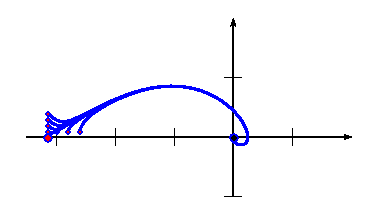
\includegraphics[width=0.7\textwidth]{ShipGlobalFlow}
   \caption{Global Properties of the Flows: All the curves starts from the repelling posture(Red) and ends at the attractive one(Blue)}
   \label{fig:globalflow}
  \end{center}
\end{figure}

 



\subsubsection*{Generalization of the Ship Example} 
This conclusion is independent of the shape, size, weight or material of the ship. 
Same wave perturbations will result in different sway motions for different ships.
As long as the qualitative structure design criteria is maintained, balancing is ``easy''.
On phase portraits,  all the ships share following properties. 
\begin{itemize}
\item one repelling point 
\item one attractive point 
\item all flows starts from repelling point and ends at the  attractive point. 
\end{itemize}


\begin{figure}[!htbp]
  \begin{center}
   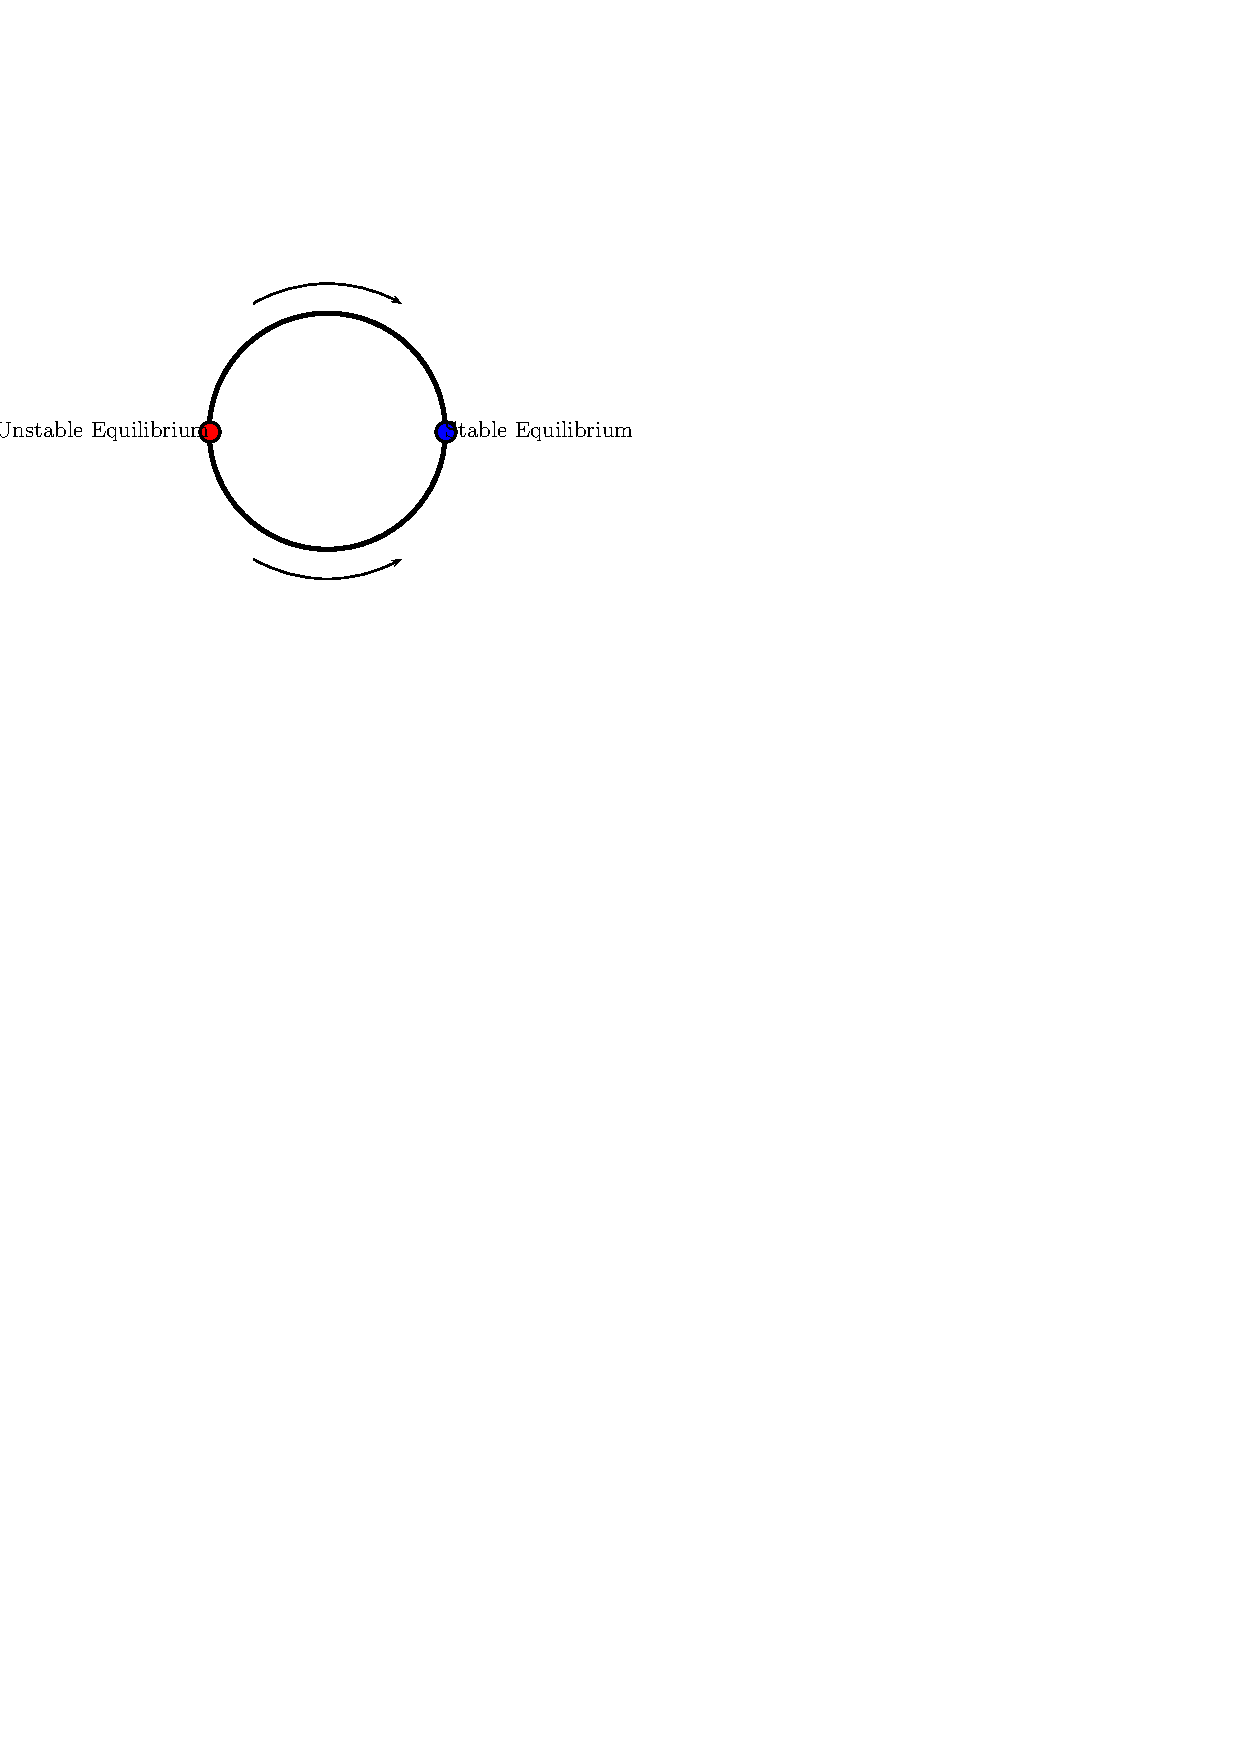
\includegraphics{topologyStructure}
   \caption{the topology  the phase portraits of ship dynamic}
   \label{fig:topologyStructure}
  \end{center}
\end{figure}

The variation of motion results from different ship design parameters is an example of \emph{system adaptation}.


\subsection{The Mass Spring System:  Symmetry Transformation}
Despite the complexity of body structure, motions of animals are executed with high accuracy in real-time.
Real-time accuracy is another puzzle in motor control, as solving the complex dynamics requires inhibitive computational cost.
In \moit, quantitative control is based on the idea of transformation, new motions are transformed from some templates.
To make motion energy efficient and natural looking, control system should choose the transformation admitted by the natural dynamics.

This ideas can be illustrated by the following mass spring example shown Figure~\ref{fig:massspring}, which captures some important properties of biological natural dynamics.
The muscle actuators are compliant and works like spring,  bones are are modelled as mass.

\begin{figure}[!htbp]
  \begin{center}
    \includegraphics[width=0.7\textwidth]{MassSpring}
    \caption{the mass spring system}
    \label{fig:massspring}
  \end{center}
\end{figure}

\subsubsection*{Dynamics}
The canonical equation of mass spring system is
\begin{equation}
\label{eq:mass-spring}
\ddot{q}+q=0.
\end{equation}
where $q$ is the offset distance.

By define the \emph{state variable}, $\state=[q,\qd]$, it can also be reformulated as
\[
\dot{\state}=F(\state)
\]

 Figure~\ref{fig:massSpringPhasePlot} shows the phase plot with two flows.


\begin{figure}[!htbp]
  \begin{center}
     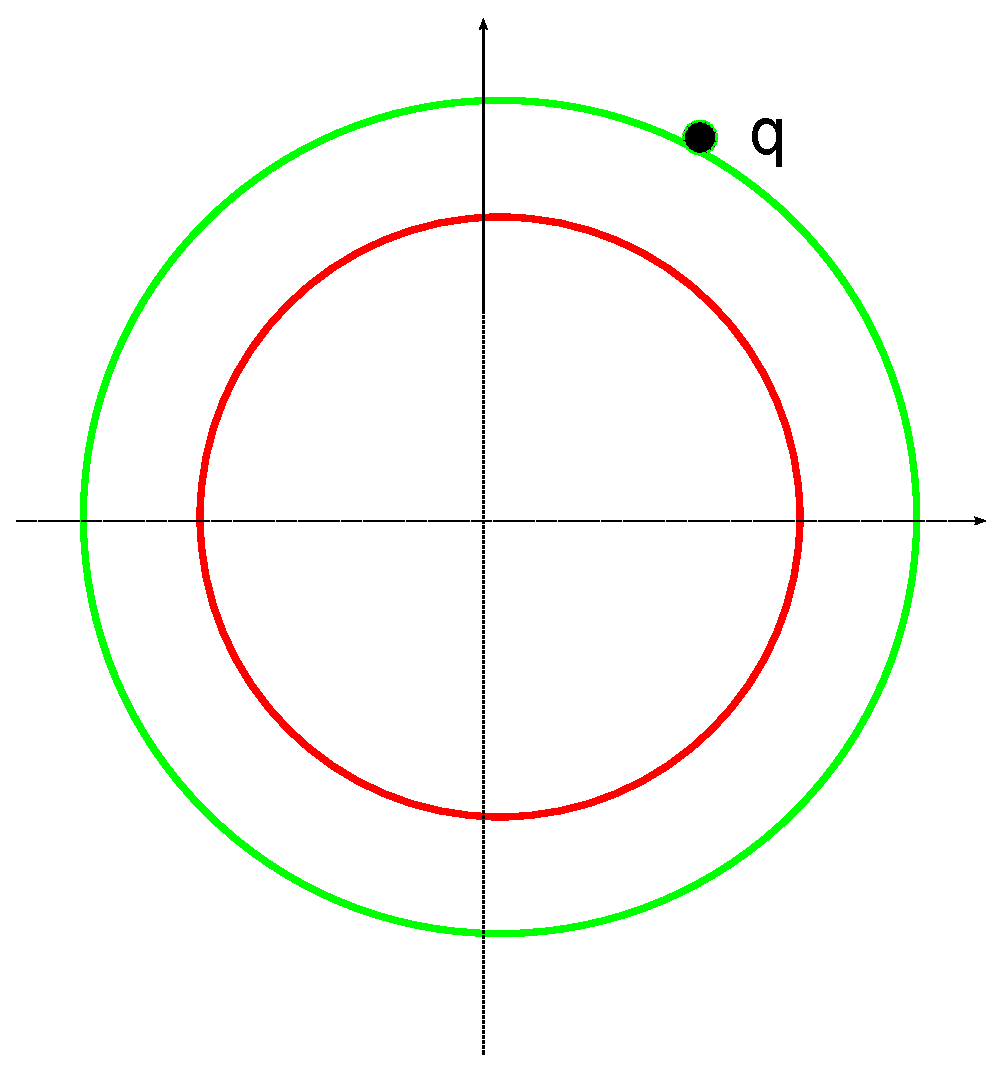
\includegraphics[width=0.5\textwidth]{MassSpringPhasePlot}
    \caption{Mass Spring Phase Plot:two motion curves are shown.The red one and the green pass through different state $\state$,$\state'$}
    \label{fig:massSpringPhasePlot}  
  \end{center}
\end{figure}

\subsubsection*{Symmetry and Transformation}
%It is highly unlikely animals can solve Equation~\ref{eq:mass-spring}.

The mass spring system has some ``symmetrical properties''.
Different flows share the same circle ``Shape''.
New flows(green) can be find by scaling the original(red) flow.

From mechanical viewpoint, this is because the flows of mass spring are energy preserving.
We can define the energy function
\[
E=\frac{1}{2}(m\qd^2+kq^2)
\]
where $k$ is the stiffness, $m$ is the mass.
When $m=1,k=1$, $E$ is a constant,suppose $E=c$,
then $q^2+\qd^2=2c$, which is the implicit function of a circle.

Given flows that pass through  $\state$.
For the state $\state^{'}$, by checking the energy, the scale transformation from red to green can be workout,then we know the future motion after $\state^{'}$.


\subsubsection*{Dynamic Perception}

The idea ``transformation and symmetry'' may shed light on dynamic perception. 
It is highly unlikely animals can solve Equation~\ref{eq:mass-spring} to understand mass spring system.
The dynamics can be encoded in a different manner: a motion template and the symmetry property.
If so, we can validate observation by applying transformation to motion templates in our memory.


Rather than working out the transformation directly,
it is better to check some property invariant under transformation.
For the mass spring system example, we can check the ``shape'' of the flow,
from differential geometrical perspective,  the curvature is invariant.
or dynamically checking the energy preserving property. 
 


Quantitative invariant properties like energy preserving or curvature of flow are called \emph{Local Motor Invariant}. 
Adaptation generated by transformation is called \emph{transform adaptation}.

\section{Contribution}

Compared with current \cms methods, the new approach has several advantages:
\begin{enumerate}
\HiItem {More Types of Adaptation}
Most dynamic method only focus on generating response motion to dynamic perturbation.
Adaptations across different characters are treated as a separate  research topic(motion retargeting).
\moit unified the theory for different adaptation, topology conjugacy  incorporate both motion re-targeting and  response  in an unified framework.
\moit can generate more types of adaptation.
\HiItem {Better Usability}.
For many \cms methods, each \dof ~is controlled independently.
When modifying controllers, animator has to modify each \dof, which is a tedious work.

In \moit, adaptation is achieved by applying transformation.
Each transformation can be parametrized by one parameter.
By specify one parameter, all \dof s are modified automatically, which is more artist friendly.

\HiItem {No Reference Motion}
\moit relies on the dynamic equation of body and environment for motion primitives.
Motion Capture Data is not needed as reference.
In situations, this method can generate new motion unlike the reference.


\HiItem {Computationally Efficient} 
This motion synthesis approach runs in real-time.
\HiItem {Motion Transition}
Dynamic motion transition are developed upon solid theory foundation.

\end{enumerate}

Because of its biological foundation,
algorithms and simulation results in \moit  might shed light into biology research.
Some conclusion and control techniques can be treated as candidate theory that needs further verification.

\begin{enumerate}
\item 
Motion Primitive is an old idea in biological research, but there is no agreement on the definition and underlying reason.
Biological research has tried identify motion primitive by exploring the neural anatomy, EMG signal or muscle activation pattern.

\moit  explains the motion primitive from dynamic viewpoint.
This theory is more complete,
besides identification, it also answers why certain motions are primitives and others are not,
how many motion primitives we have and where they come from.

\item One supporting theory of motion primitive is the muscle synergy:
Generating motion by actuating muscles, muscles are not controlled independently but worked in group. 
Many research in synergy by empirical methods. 

In \moit, when control is applied to ensure transformation, actuators are controlled in an ``synergy manner''.
\moit provide and candidate  ``synergy'' method for muscle control.

\item For the neural structure \emph{Central Pattern Generator}(\cpg) , their roles in motor control are well agreed.
While detail strategy for adjust \cpg parameters according to motor purpose is still lacking.
The \moit provides an theory for modifying the \cpg parameters with mathematical rigidity.


\item  Motion and dynamic perception mechanism of neural system is still unclear.
The motor invariant theory propose a computationally efficient mathematical machinery.
\end{enumerate}







\section{Organization of the Thesis}

This thesis is organized as follows.
 
In Chapter~\ref{chap:background}, previous research on motion synthesis and biological motor control are discussed, which are the motivation and justification of \moit.
 
In Chapter~\ref{chap:gi}, \emph{Qualitative Dynamicss} is introduced to explain motion primitives. 
Biological based  methods for maintaining the global motor invariant are developed.

Chapter~\ref{chap:li} focuses on the idea of Local Motor Invariant and Symmetry.
Lie Group theory is  introduced  to analyse the symmetry properties in motion dynamics.
Symmetry Controllers are developed for adaptation motions.
 


Chapter~\ref{chap:msf} discuss the combination problems.
For each motion primitive,  strategies are developed to preserve global and local motor invariant simultaneously.
Motion primitive transition is discussed and methods for combining motion elements into more complex motion is discussed.
As an animation system, the software architecture and work flow are discussed at the end.

Chapter~\ref{chap:gi},~\ref{chap:li},~\ref{chap:msf} lay the theoretical foundation of \moit.
Following chapters focus on application in \cms.



Chapter~\ref{chap:walk} focuses the tweaking of one primitive.
Bipedal walking is chosen, which is one of the most challenging problem for current \cms research.
Motor Invariant Theory introduce method to boost the stability and generate adaptive gaits.


In Chapter~\ref{chap:stance}, combinations of motion primitives are discussed.
A new balancing motion primitive is developed. 
Transitional motions are generated for stance to walk and walk to stance transitions.

In Chapter~\ref{chap:highdor}, extensions of motor invariant theory to more complex characters are discussed.
Three strategies are developed to simplify the problem for different situations.

This thesis ended with Chapter~\ref{chap:con}. 
After discussion of new finding of this research, some new question and ideas for graphics and neural science are proposed for further research .





%%% ----------------------------------------------------------------------


%%% Local Variables: 
%%% mode: latex
%%% TeX-master: "../thesis"
%%% End: 

